\section{Concurrencia vs. Paralelismo}

\begin{frame}{Definiciones clave}
  \begin{itemize}
    \item Concurrencia: múltiples tareas progresan de forma intercalada; ideal para E/S y ocultar latencia.
    \item Paralelismo: ejecución simultánea real en núcleos distintos; requiere hardware multiprocesador.
    \item En Python los hilos son concurrentes por el GIL; en C los hilos pueden ser concurrentes y paralelos.
  \end{itemize}
\end{frame}

\begin{frame}{Uso recomendado}
  \begin{itemize}
    \item E/S intensiva: concurrencia con hilos o async para mantener alta utilización de CPU.
    \item Carga CPU: dividir dominios de datos y mapearlos a núcleos mediante hilos nativos o procesos.
    \item Riesgos: condiciones de carrera y errores de partición (off-by-one) si no se planifica el rango de trabajo.
  \end{itemize}
\end{frame}

\begin{frame}{Ilustración conceptual}
  \begin{figure}
    \centering
    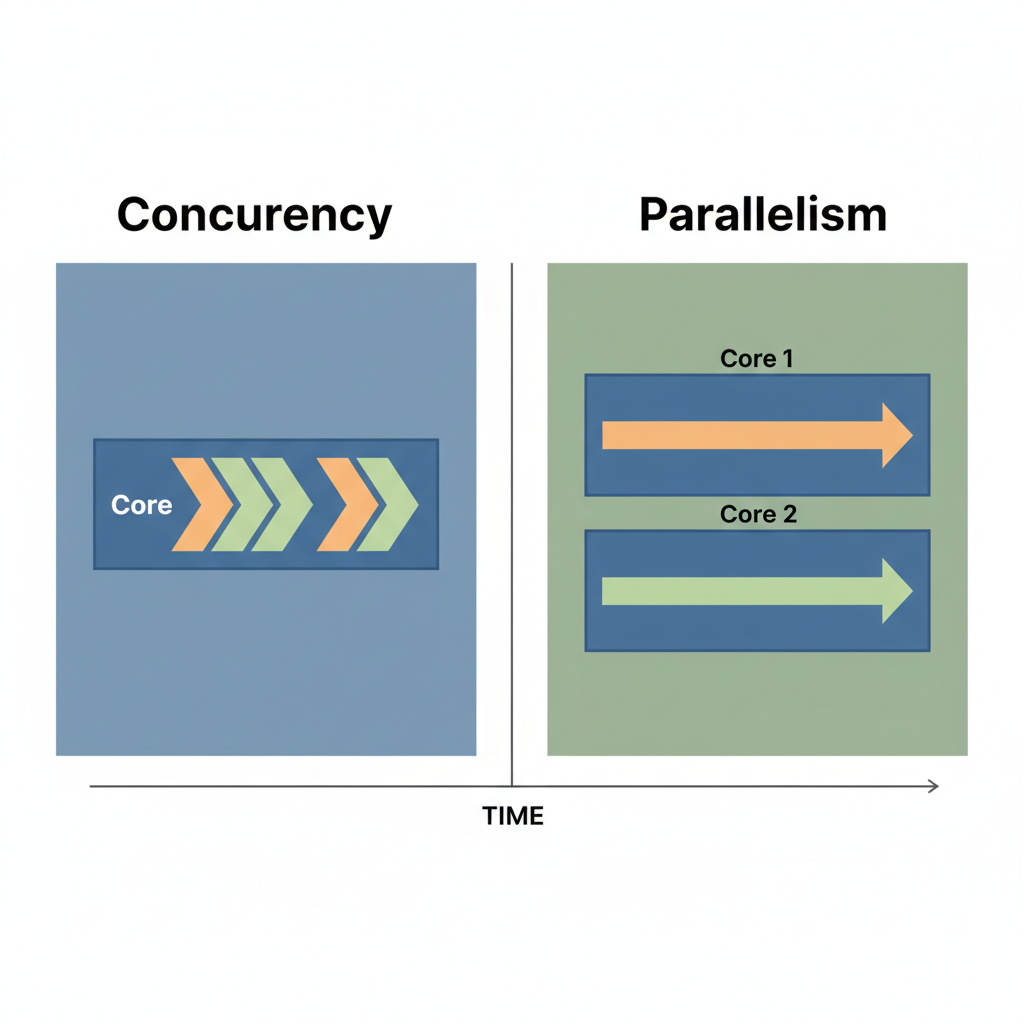
\includegraphics[height=0.6\textheight]{img/02-concurrencia-vs-paralelismo.png}
    \caption{Concurrencia vs. Paralelismo.}
  \end{figure}
\end{frame}
